\chapter{The Continuous Stored Energy Vertex Model}
%\section{The Continuous Stored Energy Vertex Model}
\label{chap:storedenergy}

\section{Introduction}

\emph{Comment: The Introduction is for now a copy and paste
of what we had in dropbox paper. It will be improved asap.}


\begin{itemize}
    \item 
\textbf{NUCLEATION GROWTH PROCESSES: A MONTE CARLO SIMULATION (1977)}

Nucleation in layers.

\item \textbf{On Abnormal Subgrain growth and the origin of recrystallization nuclei (2003)}

\url{https://www.sciencedirect.com/science/article/pii/S135964540300079X}
Abnormal (The preferential or discontinuous evolution of a few grains in a polycrystal is termed abnormal grain growth) subgrain growth (grain inside grain) was found to be a plausible nucleation mechanism for recrystallization. They are not seeded in any form, emerges spontaneously. MC method used for simulation and comparison with experimental data.

\item \textbf{Recrystallization study using two-dimensional vertex model (2005)}

\url{https://yadda.icm.edu.pl/baztech/element/bwmeta1.element.baztech-article-BSW3-0014-0007}

Initial configuration: topology, orientations and stored energy. They aim to predict texture and microstructure modification during recrystallization. Inputs for the model are deformation texture, stored energy distribution and initial microstructure obtained from experiments.
Here the stored energy is introduced because allows nucleation. New nuclei are placed at the beginning of simulation with initial stored energy zero. Two nucleation were tested: random and proportional to the stored energy of the previous grain. Prefered nucleation predicts more correct texture change. Stored energy relative units range from 3 to 6.

\item \textbf{Generalized vertex model of recrystallization - Application to -polycrystalline copper (2008)}

\url{https://www.sciencedirect.com/science/article/pii/S0927025607002819}
“It is well known that recrystallization can significantly modify the distribution of orientations (texture) inside the material and produce drastic changes of many physical properties (electrical resis- tance, internal stresses, micro-hardness, etc.)”. Stored energy values are experimentaly obtained via x rays. Comparison of SE distribution, Boundary Misorientation distribution and texture (orientation).
Disadvantages for us: Uses SE with a vertex model.
Advantages for us: They don’t analyze mathematically when a nucleation will be successful ($\Delta$ SE). They mention (at the end) that they can’t compute MDF and ODF since they have few grains. There isn’t any computational implementation discussion.

\item \textbf{On the widths of orientation gradient zones adjacent to grain boundaries (2009)}

\url{https://www.sciencedirect.com/science/article/pii/S1359646209002589}
Paper aboux experimental results of orientations in grains. Does not mention recrystallization process (they do work over recrystallized material), stored energy nor nucleation.

\item \textbf{Level set framework for the finite-element modelling of recrystallization and grain growth in polycrystalline materials (2010)}

\url{https://www.sciencedirect.com/science/article/pii/S1359646210007906}
Model implemented a set of convection-reinitialization-diffusion equations with finite elements. Nucleation is implemented by introducing new grains based on some probabilistic or deterministic criteria. The sites for nucleation can be chosen randomly, at grain boundaries or according to criteria based on previous deformation step of polycrystal. Implementation in Cimlib C++ library. Three examples to show the capabilities of the model are presented. First is the motion of a vertex given a grain with a certain stored energy and its steady state and the motion of a vertex with an unstable initial condition and uniform SE in grains that reaches a steady state also. Second, an example with 1000 grains of isotropic grain growth and Third, 100 initial grains with random stored energy distribution and 200 new grains for nucleation with SE= 0, snapshots of different process (primary recrystallization and grain growth) are shown.

\item \textbf{Monte Carlo model in metal recrystallization simulation (2011)}

\url{https://link.springer.com/article/10.1007/s12204-011-1156-x}
Again an improved MC model which aims to simulate non-homogeneous recrystallization, the model does not take in account texture, thus results on isometric grains and experimental isometric grains differ because the model does not take in account the preffered growth orientation. Simulated grain size is less than experimental results.

\item \textbf{Interplay of kinetics and microstructure in the recrystallization of pure copper: Comparing mesoscopic simulations and experiments (2012)}

\url{https://link.springer.com/article/10.1007/s11661-012-1094-8}
The simulated microstructures after recrystallization exhibit a bimodal grain-size distribution instead of the broad, monomodal grain-size distribution found in the experiments. Cellular automaton model. Something about nucleation nature “‘Nucleation’’ in recrystallization is not a fluctuation phenomenon like in (solid–solid) phase transformations. Instead, the ‘‘nuclei’’ are present already in the deformed material in the form of subgrains that can become ‘‘activated’’ or ‘‘supercritical,’’ i.e., become ‘‘nuclei,’’ if certain instability criteria are (all) fulfilled”
“double-logarithmic plot of the recrystallized fraction as function of time”

\item \textbf{Investigation of nucleation and grain growth in 2-dimensional systems by using generalized Monte Carlo simulations (2013)}

\url{https://www.sciencedirect.com/science/article/pii/S0378437113003531}

2D generalized montecarlo simulation, achieves better result locating energy minima

\item \textbf{An Extended Vertex and Crystal Plasticity Framework for Efficient Multiscale Modeling of Polycristalline Materials (2017)}

\url{https://www.sciencedirect.com/science/article/pii/S0020768317303268#bib0031}
This multiscale modeling couples extended vertex model and crystal plasticity formulation. Allows stored energy, nucleation, pinning. GPU-implementation of the crystal plasticity component. They mention that there is no model where crystal plasticity is coupled to vertex model formulation. They also mention some vertex models that only consider grain growth and do not include influence or stored energy and anisotropic grain boundary properties. They mention that Piekos does not consider pinning nor anisotropic GB properties. Topological transitions are based on minimum length  $\Delta$ (so, this could also be studied). With introduction of SE they implement topological transition to break a grain (see Piekos 2005). Nucleation is placed in TJ and along grain boundaries. They do not mention numerical limits for SE effects. Tested on copper data.
Disadvantage for us: They study a similar model and work with Physical parameters. 
Advantages for us: It is still an active research topic, they only added a GPU-implementation for a small part of the model. The code is not available. They don’t study mathematica properties of the model (effect of SE to TJ, $\Delta$ SE min for nucleation).
\end{itemize}

\subsection{Overall Review}

It seems that nucleation mechanisms and simulations are compared with textures like copper and heavily deformed structures.
Orientation distribution function and misorientation distribution are studied from experimental data.  This experimental data also is used as input for configuration in simulations in, e.g. the varied MC models.
We also found coupled variation to obtain simulation for nucleation, primary recrystallization and grain growth. This kind of models (adaptation of vertex model) required certain topological transition to be stable.
The two most important “newer” papers are:
1.- Generalized vertex model of recrystallization - Application to -polycrystalline copper (2008)
2.-An Extended Vertex and Crystal Plasticity Framework for Efficient Multiscale Modeling of Polycristalline Materials (2017)

Another important paper is: Level set framework for the finite-element modelling of recrystallization and grain growth in polycrystalline materials, because they numerically study the role of SE for a vertex but they do their mathematical analysis. This is what we did with @Alejandro S for the poster we presented. So, it is worth to explain in detail.

\section{Related work}

 \lettrine{E}{xtension} of the classic vertex model considers the introduction of an intragranular stored energy $\SE$ which plays a key role in primary recrystallization. This process can significantly modify the distribution of orientations inside the material and produce drastic changes of many physical properties like electrical resistance, internal stresses, micro-hardness, etc.\cite{pikekos2008generalized, pikekos2008stochastic}
 The local energy of a vertex $i$ considering the stored energy term can be defined as:
 \begin{equation}
     E_i(t) = \sum_{j \in \mathcal{N}_i}\left(\gamma_{i,j}\AL_{i,j}(t) + \SE_{i,j}A_{i,j}(t)\right),
 \end{equation}
 %
 where $\mathcal{N}_i$ is the set of neighbor vertices to the vertex $i$, $\AL_{i,j}$ is the arc length of the boundary formed by vertices $i$ and $j$, $\SE_{i,j}$ and $A_{i,j}$ is the stored energy and area of a grain adjacent to the boundary $i,j$ using the right-hand rule. We split the local energy between the grain boundary contribution and the grain area contribution, so:
 \begin{equation}
     E_i(t) = \sum_{j \in \mathcal{N}_i}\gamma_{i,j}\AL_{i,j}(t) + \sum_{g \in \mathcal{G}_i} \SE_{g}A_{g}(t),
 \end{equation}
 %
 where $\mathcal{G}_i$ is the set of grains associated to vertex $i$. Now, we could define the total energy of the system as:
 \begin{equation}
     E(t) = \sum_{k \in \boundaries}\gamma_{k}\AL_{k}(t) + 
     \sum_{g \in \mathcal{G}} \SE_{g}A_{g}(t),
     \label{eq:SEtotalenergy}
 \end{equation}
 %
 where $\boundaries$ is the set of all the boundaries in the grain structure
 and $\mathcal{G}=\bigcup_i \mathcal{G}_i$ is the set of grains.
 So, now we could decompose the contribution
 from each vertex to the total energy as follows,
 %
 \begin{equation}
     \widehat{E}_i(t) = \sum_{j \in \mathcal{N}_i}\gamma_{i,j}\dfrac{\AL_{i,j}(t)}{2} + \sum_{g \in \mathcal{G}_i} \SE_{g}\dfrac{A_{g}(t)}{\ns(g)},
         \label{eq:SEvertexenergy}
 \end{equation}
 %
 where $\ns(g)$ is the number of sides (or class) of grain $g$. 
 This allows us to build the total energy
 as the sum of the contribution of each vertex
 such that we ensure we only consider once
 each grain boundary contribution and also consider
 once each grain contribution, thus,
 %
\begin{align*}
     \sum_{i \in \mathcal{N}}\widehat{E}_i(t) &=
     \sum_{i \in \mathcal{N}}\left(
     \sum_{j \in \mathcal{N}_i}\gamma_{i,j}\dfrac{\AL_{i,j}(t)}{2} + \sum_{g \in \mathcal{G}_i} \SE_{g}\dfrac{A_{g}(t)}{\ns(g)}\right) \\
     &=
     \underbrace{\sum_{i \in \mathcal{N}}\left(
     \sum_{j \in \mathcal{N}_i}\gamma_{i,j}\dfrac{\AL_{i,j}(t)}{2}\right)}_{(a)}  + 
     \underbrace{\sum_{i \in \mathcal{N}}\left(\sum_{g \in \mathcal{G}_i} \SE_{g}\dfrac{A_{g}(t)}{\ns(g)}\right)}_{(b)}
 \end{align*}
In order to solve $(a)$ we need to understand which elements are being counted. The outer sum takes all the vertices and the inner sum takes the neighbor vertices of each vertex. Consider the expanded terms for some vertex $k$:
\begin{equation*} \gamma_{k,j_1} \frac{\AL_{k,j_1}(t)}{2} + 
\gamma_{k,j_2} \frac{\AL_{k,j_2}(t)}{2} +
\gamma_{k,j_3} \frac{\AL_{k,j_3}(t)}{2},
\end{equation*}
where $j_1, j_2, j_3$ are the three neighbor vertices of vertex $k$. Let's see now the terms associated to one of these vertices, for example $j_1$:
\begin{equation*} \gamma_{j_1,k} \frac{\AL_{j_1,k}(t)}{2} + 
\gamma_{j_1,j_{12}} \frac{\AL_{j_1,j_{12}}(t)}{2} +
\gamma_{j_1,j_{13}} \frac{\AL_{j_1,j_{13}}(t)}{2}.
\end{equation*}
It is clear that for each vertex we are counting the energy associated to each boundary twice, each per vertex in a boundary. This justifies the introduction of the term $1/2$ in $\widehat{E}_i(t)$. The analysis to solve $(b)$ is similar. The inner sum of here runs over the grains related to vertex $i$. We can build a similar example starting from a vertex $k$ and counting the three stored energy terms related as:
\begin{equation*}
    \SE_{g_1} \frac{A_{g_1}(t)}{\ns(g_1)}+
    \SE_{g_2} \frac{A_{g_2}(t)}{\ns(g_2)}+
    \SE_{g_3} \frac{A_{g_3}(t)}{\ns(g_3)}
\end{equation*}
Consider now that $g_1$ has $\ns(g_1)$ vertices. We already know that $k$ is a vertex of $g_1$, the terms related to the $\ns(g_1) -1 $ remaining vertices must have a term $\SE_{g_1} \dfrac{A_{g_1}(t)}{\ns(g_1)}$ and thus we are summing in $(b)$ the same term $\ns(g_1)$ times. Of course, for any grain $g$ the times the related stored energy term is being added $\ns(g)$ times. This justifies the introduction of the term $1/\ns(g)$. Finally we can map the sum in order to count boundaries and grains. Each term related to a boundary is counted twice and each term related to a grain is counted $\ns(g)$ times and we can recover an expression for the total energy of the system as:

 \begin{align*}
     \sum_{i \in \mathcal{N}}\widehat{E}_i(t) &= \sum_{k \in \boundaries}2\,\gamma_{k}\dfrac{\AL_{k}(t)}{2} + 
     \sum_{g \in \mathcal{G}} \ns(g)\,\SE_{g}\dfrac{A_{g}(t)}{\ns(g)}\\
      &= \sum_{k \in \boundaries}\gamma_{k}\AL_{k}(t) + 
     \sum_{g \in \mathcal{G}} \SE_{g}A_{g}(t) \nonumber\\
     &=E(t).
 \end{align*}
 %
 %
Notice that $\widehat{E}_i(t)$ is different
from $E_i(t)$.
%If we had just added up $E_i(t)$ to build
%the total energy, we would have counted
%each grain boundary contribution twice
%and each grain contribution proportional
%to the number of sides of each grain.

The boundary arc length $\AL$ and grain area $A$ can be seen as function of the vertices positions $\{\x_i\}$. Rewriting \eqref{eq:SEvertexenergy} marking this dependence as:
\begin{equation}
    \widehat{E}_i(\x(t)) = \sum_{j \in \mathcal{N}_i}\gamma_{i,j}\dfrac{\AL_{i,j}(\x)}{2} + \sum_{g \in \mathcal{G}_i} \SE_{g}\dfrac{A_{g}(\x)}{\ns(g)},\label{eq:vertexenergy}
\end{equation}
The evolution of the system, considering the stored energy term, such that it decreases energy
is obtain by a gradient descent method, so
$\dotx_i(t) = -\dfrac{\partial E}{\partial \x_i}$ for each vertex.

\section{Implementation}
Computing the velocity of each vertex is actually the computation of the gradient $\nabla_{\x}E$. 
Here we propose a matrix-free approach to approximate the gradient.
The main advantage of this approach is that it only needs the implementation of computation of the energy of the system, this simplifies enormously the bookkeeping we would need to handle this task.

A convenient approximation to compute $\dfrac{\partial E(\X)}{\partial \x_i}$ is to perform a matrix-free approach. 
Consider the vector $\X \in \mathbb{R}^{2n}$ of stacked components of $\x_i =(x_i, y_i)$, this is $\X = (x_1, x_2, \cdots, x_n, y_1, y_2, \cdots, y_n)^T$ where $n$ is the total number of triple junctions. 
Each $k$-th component of the gradient for this vector, say $\dfrac{\partial E(\X)}{\partial \X_k}$ is approximated by:
\begin{equation}
    \frac{\partial E(\X)}{\partial \X_k} \approx 
    \frac{E(\X + \varepsilon\,  \ei{k}) - E(\X)}{\varepsilon},
    \label{eq:partialE}
\end{equation}
where $\ei{k}$ is the $k$-th canonical vector in $\mathbb{R}^{2n}$. 
The numerical evaluation of this approximation implies that the energy of the system must be recomputed twice for each vertex, and according to \eqref{eq:SEtotalenergy} this means to recompute each individual vertex energy each time.
Fortunately, 
%this can improved.
this can be handled efficiently by pointing out which terms will change after the perturbation.

This quadratic cost required for a naive implementation is not real in practice. 
%as we explain here. 
A more detailed analysis shows that the perturbation only affects the $x$ or $y$ component of a vertex $\x_i$, which implies that only the three related grain areas and the three grain boundary arc-lengths will change as shown in Figure \ref{fig:delta_energy}.
%Thus the total energy changes only for the vertex $i$ and its three neighbors as shown in Figure \ref{fig:delta_energy}.
Thus the total energy is modified by each vertex that has a perturbed arc-length or area, that is, for each vertex belonging to the grains of $\x_i$.

\begin{figure}[t]
    \centering
    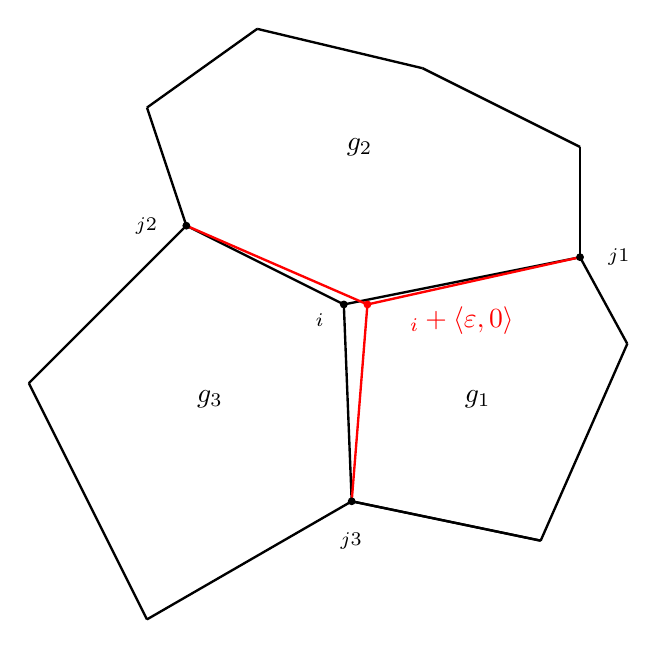
\begin{tikzpicture}
        % boundaries
        % grain 1
        \draw[line width=0.3mm, black] (0,0) -- (3,0.6);
        \draw[line width=0.3mm, black] (3,0.6) -- (3.6,-0.5);
        \draw[line width=0.3mm, black] (3.6,-0.5) -- (2.5, -3);
        \draw[line width=0.3mm, black] (2.5,-3) -- (0.1, -2.5);
        \draw[line width=0.3mm, black] (0.1,-2.5) -- (0,0);
        % grain 2
        \draw[line width=0.3mm, black] (2.5,-3) -- (0.1, -2.5);
        \draw[line width=0.3mm, black] (0,0) -- (-2, 1);
        \draw[line width=0.3mm, black] (-2,1) -- (-4, -1);
        \draw[line width=0.3mm, black] (-4,-1) -- (-2.5, -4);
        \draw[line width=0.3mm, black] (-2.5,-4) -- (0.1, -2.5);
        % grain 3
        \draw[line width=0.3mm, black] (-2,1) -- (-2.5, 2.5);
        \draw[line width=0.3mm, black] (-2.5,2.5) -- (-1.1, 3.5);
        \draw[line width=0.3mm, black] (-1.1,3.5) -- (1,3);
        \draw[line width=0.3mm, black] (1,3) -- (3,2);
        \draw[line width=0.3mm, black] (3,2) -- (3,0.6);
        % Perturbed data
        \draw[line width=0.3mm, red] (0.3,0) -- (3,0.6);
        \draw[line width=0.3mm, red] (0.3,0) -- (-2,1);
        \draw[line width=0.3mm, red] (0.3,0) -- (0.1,-2.5);
        % vertices
        \filldraw [black] (0,0) circle (1.2pt);
        \filldraw [black] (3,0.6) circle (1.2pt);
        \filldraw [black] (-2,1) circle (1.2pt);
        \filldraw [black] (0.1,-2.5) circle (1.2pt);
        \filldraw [red] (0.3,0) circle (1.2pt);
        \node[draw=none, color=black] at (-0.3, -0.2) {$\x_i$};
        \node[draw=none, color=red] at (1.5, -0.2) {$\x_i + \langle \varepsilon,0 \rangle$};
        \node[draw=none, color=black] at (3.5, 0.6) {$\x_{j1}$};
        \node[draw=none, color=black] at (-2.5, 1) {$\x_{j2}$};
        \node[draw=none, color=black] at (0.1, -3) {$\x_{j3}$};
        \node[draw=none, color=black] at (0.2, 2) {$g_2$};
        \node[draw=none, color=black] at (-1.7, -1.2) {$g_3$};
        \node[draw=none, color=black] at (1.7, -1.2) {$g_1$};
    \end{tikzpicture}
    \caption[Vertex perturbation in Stored Energy model]{Scheme of vertex modifying surrounding grains and boundaries. Arc lengths and grain areas are modified.}
    \label{fig:delta_energy}
\end{figure}

%\begin{figure}[t]
    %\centering
    %\includegraphics[scale=0.5]{scheme.pdf}
    %\caption[Vertex perturbation in Stored Energy model]{Scheme of vertex modifying surrounding grains and boundaries. Arc lengths and grain areas are modified.}
    %\label{fig:delta_energy}
%\end{figure}

So, instead of recompute the $n$ vertex energies for each one of the $2n$ components of the gradient, we can check directly the difference of energies given by the perturbation. 
Expanding the difference of energies from \eqref{eq:partialE} and taking into account that the perturbation effect is local, we obtain:
% \begin{align}
%     E(\X+\varepsilon\,  \ei{k}) - E(\X) &=  \widehat{E}_i(\X+\varepsilon\,  \ei{k}) - \widehat{E}_i(\X) + \sum_{j \in \mathcal{N}_i}  \widehat{E}_{j}(\X+\varepsilon\,  \ei{k}) - \widehat{E}_{j}(\X)
% \end{align}
\begin{align*}
    E(\X+\varepsilon\,  \ei{k}) - E(\X) &=  
    \sum_{k \in \boundaries}\gamma_{k}\Delta{\AL}_{k}(t) + 
     \sum_{g \in \mathcal{G}} \SE_{g}\Delta{A}_{g}(t)\\
     &=\sum_{k \in \{j_1,j_2,j_3\}}\gamma_{k}\Delta{\AL}_{k}(t)
     +\sum_{g \in \{g_1,g_2,g_3\}} \SE_{g}\Delta{A}_{g}(t)
\end{align*}
% OLD Version
{
% The energy difference holds some common terms. For example $\widehat{E}_i(\X+\varepsilon\,  \ei{k})$ has the modified arc-lengths and areas considering that $\x_i$ moved but the stored energies and boundary energies remains constant in this time-step, thus we can use \eqref{eq:vertexenergy} and factorize $\widehat{E}_i(\X+\varepsilon\,  \ei{k}) - \widehat{E}_i(\X)$ by these constants.
% \begin{equation*}
%      \widehat{E}_i(\X+\varepsilon\,  \ei{k}) -  \widehat{E}_i(\X)=  \sum_{j \in \mathcal{N}_i}  \gamma_{i, j} \frac{(\Tilde{\AL}_{i,j} - \AL_{i,j})}{2} + \sum_{g \in \mathcal{G}_i} \SE_{g}\frac{(\Tilde{A}_{g} - A_{g})}{\ns(g)} ,
% \end{equation*}
% where $\Tilde{\AL}_{i,j}$ is the perturbed arc length for vertices $i$ and $j$ and $\Tilde{A}_{g}$ is the perturbed area of the grain $g$. The other energies terms related to neighbor vertices can be analyzed as follows. The difference $\widehat{E}_{j_1}(\X+\varepsilon\,  \ei{k}) - \widehat{E}_{j_1}(\X)$ resides in the contribution of the modified areas $\Tilde{A}_{g_1}, \Tilde{A}_{g_2}$ and the arc length $\Tilde{\AL}_{i, j_1}$. The rest of the terms remains the same in each energy term and thus are canceled, therefore:
% \begin{equation}
%     \widehat{E}_{j_1}(\X+\varepsilon\,  \ei{k}) - \widehat{E}_{j_1}(\X) = \gamma_{i,j_1}\frac{(\Tilde{\AL}_{i, j_1} - \AL_{i, j_1})}{2} + \SE_{g_1}\frac{(\Tilde{A}_{g_1} - A_{g_1})}{\ns(g_1)} + \SE_{g_2}\frac{(\Tilde{A}_{g_2} - A_{g_2})}{\ns(g_2)}
% \end{equation}
% The remaining energy differences for each neighboring vertex can be obtained analogously:
% \begin{align}
%     \widehat{E}_{j_2}(\X+\varepsilon\,  \ei{k}) - \widehat{E}_{j_2}(\X) &= \gamma_{i,j_2}\frac{(\Tilde{\AL}_{i, j_2} - \AL_{i, j_2})}{2} + \SE_{g_2}\frac{(\Tilde{A}_{g_2} - A_{g_2})}{\ns(g_2)} + \SE_{g_3}\frac{(\Tilde{A}_{g_3} - A_{g_3})}{\ns(g_3)}\\
%     \widehat{E}_{j_3}(\X+\varepsilon\,  \ei{k}) - \widehat{E}_{j_3}(\X) &= \gamma_{i,j_3}\frac{(\Tilde{\AL}_{i, j_3} - \AL_{i, j_3})}{2} + \SE_{g_3}\frac{(\Tilde{A}_{g_3} - A_{g_3})}{\ns(g_3)} + \SE_{g_1}\frac{(\Tilde{A}_{g_1} - A_{g_1})}{\ns(g_1)}
% \end{align}
% Notice the common terms in all the energy differences. Adding them up we obtain that:
% \begin{align}
%  \widehat{E}(\X+\varepsilon\,  \ei{k}) - \widehat{E}(\X) &= \gamma_{i,j_1} \Delta \AL_{i, j_1} + \gamma_{i,j_2} \Delta \AL_{i, j_2} + \gamma_{i,j_3} \Delta \AL_{i, j_3} \nonumber\\
%  &+ 3\left( \SE_{g_1}\frac{\Delta A_{g_1}}{\ns(g_1)} + \SE_{g_2}\frac{\Delta A_{g_2}}{\ns(g_2)} + \SE_{g_3}\frac{\Delta A_{g_3}}{\ns(g_3)}\right).
%  \label{eq:diffenergy}
% \end{align}
% Therefore we just need to compute the new arc lengths and areas and their differences.
}
% New version
Now, diving by $\varepsilon$ we obtain \eqref{eq:partialE},
\begin{align*}
    \dfrac{E(\X+\varepsilon\,  \ei{k}) - E(\X)}{\varepsilon} &=  
    \sum_{k \in \{j_1,j_2,j_3\}}\gamma_{k}\dfrac{\Delta{\AL}_{k}(t)}{\varepsilon}
     +\sum_{g \in \{g_1,g_2,g_3\}} \SE_{g}\dfrac{\Delta{A}_{g}(t)}{\varepsilon}
\end{align*}

Moreover, each estimation of the gradient can be computed in parallel maintaining the local information of temporal areas and arc lengths without overwriting data.

\section{Effect of Scale and Stored Energy}
Consider a bounded domain where three grains coexists, two of them have the same stored energy $\SE_1$ and the third has a different stored energy $\SE_2$ as shown in Figure \ref{fig:segrains}. 

\begin{figure}
    \centering
    \includegraphics[scale=0.5]{figures/SE_analysis.pdf}
    \caption[Configuration of three grains with different values of stored energy and a vertex with one degree of freedom]{Configuration of three grains with different values of stored energy and a vertex with one degree of freedom (red dot). Initially the dot is placed at $(1,\frac{b}{2})$.}
    \label{fig:segrains}
\end{figure}

To measure the effect of the stored energy and the scale of the grains we let the central vertex of coordinates $(x,\frac{b}{2})$ to freely move along $x$-axis. Let $A_1, A_2$ the areas of the grains with stored energy $\SE_1$ and $A_3$ the area of the grain with stored energy $SE_2$. Grain areas can be explicitly computed as:
\begin{align}
    A_1 &= A_2 = \frac{b(1+x)}{4} & A_3 = ab - \frac{b(1+x)}{2}
    \label{eq:SEareas}
\end{align}
We can compute each individual stored energy based on \eqref{eq:vertexenergy}. Grain class for $A_1$ and $A_3$ is four and for $A_3$ is five. Notice that in this domain, boundaries at the edges are not counted twice per grain, thus they are not divided by 2. 
\begin{align*}
\widehat{E}_0 &= \widehat{E}_3 = 1+\frac{b}{2} + \SE_1\frac{b(1+x)}{16}\\
\widehat{E}_1 &= \widehat{E}_2 = a - 1 + b + \SE_2 \frac{a b - \frac{b (1 + x)}{2}}{5}\\
\widehat{E}_4 &= b + \frac{x}{2} + \SE\frac{A_1}{2}\\
\widehat{E}_5 &= \widehat{E}_6 = a + \frac{\sqrt{(x-1)^2 + (b/2)^2}}{2} + \SE_1\frac{b(1+x)}{16} + \SE_2\frac{ab - \frac{b (1 + x)}{2}}{5}\\
\widehat{E}_6 &= \frac{x}{2} + \sqrt{(x-1)^2 + (b/2)^2} + \SE_1\frac{b (1 + x)}{8} + \SE_2 \frac{a b - \frac{b (1 + x)}{2} }{5}
\end{align*}
If we add up all the individual energy terms and replace the definitions of areas in \eqref{eq:SEareas} the total energy becomes:
\begin{equation}
    E = \sqrt{b^2 + 4 (-1 + x)^2} + x + a (4 + b\SE_2) + 
 \frac{b (8 + \SE_1(x+1) - \SE_2(1 + x))}{2}
    \label{eq:SEtotalenergyexample}
\end{equation}
If we derivate \eqref{eq:SEtotalenergyexample} with respect to $x$ we obtain:
\begin{equation}
    \frac{dE}{dx} = 1 + \frac{4 (x-1)}{\sqrt{b^2 + 4 (x-1)^2}} - \frac{b \Delta \SE}{2}
    \label{eq:deltaSE}
\end{equation}
where $\Delta \SE = \SE_2 - \SE_1$. Thus, the motion of the central vertex is influenced solely by the difference of stored energies and the height of the domain $b$. Domain width $a$ does not affect the steady state position. The steady state can be found making \eqref{eq:deltaSE} equal to 0, which yields the following roots.
\begin{equation}
    x=\frac{ -24 + 2 b \Delta \SE  (b \Delta \SE -4) \pm \sqrt{-b^2 (b \Delta \SE -6) (b \Delta \SE -2)^2 (b \Delta \SE +2)}}{2 (b \Delta \SE -6) (b \Delta \SE +2)}.
    \label{eq:xpos_steady}
\end{equation}
Under isotropic conditions of stored energy the domain height $b$ conditions the position of the steady state which is at:
\begin{equation*}
    x_{\text{steady}} = 1 - \frac{b}{2\sqrt{3}}.
\end{equation*}
By analyzing the obtained roots only some solutions will have physical sense. The critical point, assuming $\Delta \SE > 0$ is just before the squared root in \eqref{eq:xpos_steady} becomes complex at $b\Delta \SE = 6$ and solutions with $b \Delta \SE < 6$ will be real and will be valid steady states, as shown in Figure \ref{fig:SE_stability}. From the numerical point of view several experiments were performed by estimating $\dfrac{dE}{dx}$ with the matrix-free approach. As this approach will not capture complex solutions, from $b\Delta SE \geq 6$ the solutions become unstable and unbounded, as shown in Figure \ref{fig:SE_experiments}.

\begin{figure}
    \centering
    \includegraphics[scale=0.6]{figures/SE_stability.pdf}
    \caption{Stability regions for the relation of $b$ and $\Delta \SE$ in the three grains experiment.}
    \label{fig:SE_stability}
\end{figure}

The concept of stability here refers to the interpretation of the vertex position in the domain. If the vertex stays inside the three grains we say that is an steady state. If the vertex penetrates a boundary the configuration is unstable since there is no physical meaning for that configuration. Figures \ref{fig:SE_stability_SE0} and \ref{fig:SE_stability_SE15} shows two valid steady states. Figure \ref{fig:SE_stability_SE0} shows the steady state when there is isotropic configuration of stored energy, therefore the steady state is reached at dihedral angle $2\pi/3$. In presence of stored energy anisotropy the steady state is situated away from the isotropic steady state as shown in Figure \ref{fig:SE_stability_SE15}. Again, when $b\Delta \SE \geq 6$ the solution becomes unbounded.

\begin{figure}
    \centering
    \includegraphics[scale=0.5]{figures/SE_analysis_SE0.pdf}
    \caption{Steady state of grain configuration with $\SE_1 = \SE_2$.}
    \label{fig:SE_stability_SE0}
\end{figure}

\begin{figure}
    \centering
    \includegraphics[scale=0.5]{figures/SE_analysis_SE1dot5.pdf}
    \caption{Steady state of grain configuration with $\SE_1 < \SE_2$}
    \label{fig:SE_stability_SE15}
\end{figure}
 
This estimation can be used as an upper bound for numerical simulations of this model, ensuring that no grains will suffer from instabilities. The interpretation is that the parameter $b$ of this study can be somewhat compared to boundaries arc lengths. We can take each arc length and the difference of stored energy of the shared boundary and check the distribution of values for the product $\AL \Delta \SE$. We interpret that this distribution must be bounded to ensure stable simulations.

\begin{figure}
    \centering
    \includegraphics[scale=0.6]{figures/SE_experiments.pdf}
    \caption[Convergence of steady states for a fixed value of $b$ and different values of $\Delta SE$]{Convergence of steady states for a fixed value of $b$ and different values of $\Delta SE$. Values of $\Delta SE \geq 6$ become unbounded.}
    \label{fig:SE_experiments}
\end{figure}

\section{Nucleation Process}
In order to allow nucleation in vertex model, a new grain can be placed in a suitable location such that its growth also decreases the energy of the system. Consider a bounded domain box of sides $a$ centered at $(0,0)$ with four grains, three grains have the same stored energy $\SE_1$ and a fourth grain that will be nucleated centered in the middle of the box with stored energy $\SE_2$ as shown in Figure \ref{fig:SE_nucleation}. Similar to the analysis of the effect of scale and stored energy, this experiment shows which basic conditions are necessary for nucleation as a function of the stored energies involved.

The shape of the nucleated grain is initially a equilateral triangle centered at the origin of the coordinate system. The triangle is parametrized as if it were inscribed into a circle of radius $r$. Let $A_1, A_2$ the areas of the Grain areas can be explicitly computed in function of $r$ as:
\begin{align*}
A_{\text{nucl.}} &= \frac{\sqrt{3}r^2}{4} \\
A_1 = A_2 &= \frac{a^{2}}{24} \left(\sqrt{3} + 6\right)\\ A_3 &= - \frac{\sqrt{3} a^{2}}{12} + \frac{a^{2}}{2} - \frac{\sqrt{3} r^{2}}{4}
\end{align*}

\begin{figure}
    \centering
    \includegraphics[scale=0.65]{figures/SE_nucleation.pdf}
    \caption{Configuration of a nucleated grain generated at a vertex shared by three grains.}
    \label{fig:SE_nucleation}
\end{figure}

In a similar fashion as the previous experiment we compute each energy vertex and add them up to obtain the total energy of the grain system as:
\begin{equation*}
    \frac{1}{60} \left(a \left(\left(\sqrt{3}+6\right) a \epsilon +15 \gamma \right)+5 r \left(12 \sqrt{3} \beta -6 \gamma +\sqrt{3} \eta  r\right)\right)
\end{equation*}

\section{Nucleation Process 2 - Adding a 3-side grain
and letting it grow}

\begin{figure}
    \centering
       \begin{tikzpicture}
        % coordinates
        \coordinate (x1) at (0,-0.5);
        \coordinate (x2) at (0,2.1);
        \coordinate (x3) at (-2,-2.3);
        \coordinate (x4) at (2, -2.3);
        % boundaries
        \draw[line width=0.4mm, red] (x1) -- (x2);
        \draw[line width=0.4mm, red] (x1) -- (x3);
        \draw[line width=0.4mm, red] (x1) -- (x4);
        \draw[line width=0.4mm, black!10!green] (x2) -- (x3);
        \draw[line width=0.4mm, black!10!green] (x3) -- (x4);
        \draw[line width=0.4mm, black!10!green] (x2) -- (x4);
        
        % vertices
        \filldraw [black] (x1) circle (1.5pt);
        \filldraw [black] (x2) circle (1.5pt);
        \filldraw [black] (x3) circle (1.5pt);
        \filldraw [black] (x4) circle (1.5pt);
        
        % Text
        \node[draw=none, color=black, below] at (x1) {$\x_{1}$};
        \node[draw=none, color=black, above] at (x2) {$\x_{2}$};
        \node[draw=none, color=black, below] at (x3) {$\x_{3}$};
        \node[draw=none, color=black, below] at (x4) {$\x_{4}$};
        
        \node[draw=none, color=black, right] at ($(x2)!0.5!(x4)$) {$\AL_{2,4}$};
        \node[draw=none, color=black,left] at ($(x2)!0.5!(x3)$) {$\AL_{2,3}$};
        \node[draw=none, color=black, below] at ($(x3)!0.5!(x4)$) {$\AL_{3,4}$};
        
        \node[draw=none, color=black, right] at ($(x1)!0.35!(x2)$) {$\AL_{1,2}$};
        \node[draw=none, color=black, above] at ($(x1)!0.45!(x3)$) {$\AL_{1,3}$};
        \node[draw=none, color=black, above] at ($(x1)!0.45!(x4)$) {$\AL_{1,4}$};
        
        \node[draw=none, color=black] at ($0.33*(x1)+0.33*(x4)+0.33*(x2)$) {$\color{red}{A_{1}}$};
        \node[draw=none, color=black] at ($0.33*(x1)+0.33*(x2)+0.33*(x3)$) {$\color{red}{A_{2}}$};
        \node[draw=none, color=black] at ($0.33*(x1)+0.33*(x3)+0.33*(x4)$) {$\color{red}{A_{3}}$};
    \end{tikzpicture}
    %\includegraphics[scale=0.4]{figures/nucleation2.pdf}
    \caption{Sketch of energies associated to a 3-side grain before and after it is nucleated. Red shows what it is going to be removed and green what it is going to be added.}
    \label{fig:SE_nucleation2}
\end{figure}

The nucleation process can be classified as a new type of topological change in the system, considering the already well-known topological changes: flipping and  grain removal.
As usual, this new type of topological change should be energy decreasing, otherwise, it would 
induce the removal of the nucleated grain.
To analyze this topological change, we propose the following sketch, see Figure \ref{fig:SE_nucleation2}.
In this sketch we observe what we call
the current configuration of energy $E_0^{\triangle}$, in red, and a candidate configuration of energy $E_1^{\triangle}$.
The main idea is that for a candidate vertex $\x_1$, where we could perform a nucleation,
we can explicitly compute the difference of energy
before and after the nucleation, i.e. $\Delta E^{\triangle}=E_1^{\triangle}-E_0^{\triangle}$. 
So, as long as the difference is negative we can conclude that nucleation will be successful.
%In this case we have the following configuration of energies,
Thus, the $\Delta E^{\triangle}$ is as follows,
\begin{align}
    E_0^{\triangle} &= \gamma_{1,2}\,\AL_{1,2}
    +\gamma_{1,3}\,\AL_{1,3}+\gamma_{1,4}\,\AL_{1,4}
    +\SE_1\,A_1+\SE_2\,A_2+\SE_3\,A_3,\nonumber\\
    E_1^{\triangle} &= \gamma_{2,4}\,\AL_{2,4}
    +\gamma_{2,3}\,\AL_{2,3}+\gamma_{3,4}\,\AL_{3,4},\nonumber\\
    \Delta E^{\triangle} &= E_1^{\triangle}-E_0^{\triangle},\label{eq:Delta_E_Nucleation}
\end{align}
where $\x_i$ are the coordinates of the vertex $i$ for $i\in\{1,2,3,4\}$, 
$\AL_{i,j}$ is the arc-length from vertex $\x_i$ to vertex $\x_{j}$, $\gamma_{i,j}$ is the grain boundary energy from vertex $\x_i$ to vertex $\x_{j}$,  
$A_1$ is the area of grain with vertices $\{\x_1,\x_4,\x_2\}$,
$A_2$ is the area of grain with vertices $\{\x_1,\x_2,\x_3\}$,
$A_3$ is the area of grain with vertices $\{\x_1,\x_3,\x_4\}$,
and $\SE_k$ is the store energy of the grain associated to $A_k$ for $k\in \{1,2,3\}$.

\subsection{A Symmetric Nucleation Analysis}

To gain insight in the general conditions for allowing nucleation, we will consider a particular case.
Specifically, we will consider isotropic grain boundary energy $\gamma$, i.e. $\gamma=1$,
$\AL_{1,i}=r$ for $i\in\{2,3,4\}$
$\AL_{2,4}=L$, $\AL_{2,3}=L$, $\AL_{3,4}=L$, and dihedral angle of $120^\circ$.
This leads us to the following simplification
of equation \eqref{eq:Delta_E_Nucleation},
\begin{align*}
    \Delta E^{\triangle} &=
    3\,L-3\,r-
    \underbrace{(\SE_1+\SE_2+\SE_3)}_{\displaystyle{\bar{\SE}}}\,A.
\end{align*}
Moreover, due to symmetry, we have that $L=\sqrt{3}\,r$ and $A=\frac{\sqrt{3}}{4}\,r^2$. 
Plugging it in we obtain,
\begin{align*}
    \Delta E^{\triangle} &=
    3\,\sqrt{3}\,r-3\,r-
    \bar{\SE}\,\frac{\sqrt{3}}{4}\,r^2\\
    &=3\,r\,\left(\sqrt{3}-1-\frac{\sqrt{3}}{12}\,\bar{\SE}\,r\right).
\end{align*}
From which we obtain there are two critical points
with $\bar{\SE}\neq 0$, these are $r_0=0$ and 
$r_c=\dfrac{4\,(3 - \sqrt{3})}{\bar{\SE}}\approx5.071796\,(\SE_1+\SE_2+\SE_3)^{-1}$.
The first critical point $r_0=0$ indicates that making
a nucleation of area $0$ will add $0$ energy, which
is correct but we are not interested in that case.
On the other hand, the second critical point
is the one we are interested, 
$r_c \approx 5.071796 \,\bar{\SE}^{-1}$,
since from that point on we ensure we are
not increasing the energy of the system and will
let the nucleated grain to grow.
%
\begin{figure}
    \centering
    %%\includegraphics[scale=0.8]{figures/DeltaE_E10.pdf}
    \includegraphics[scale=0.6]{figures/DeltaETriangle.pdf}
    \caption{Plot of $\Delta E^{\triangle}$ symmetric with $\bar{\SE}=\SE_1+\SE_2+\SE_3=18$.}
    \label{fig:DeltaSE_E6}
\end{figure}

In Figure \ref{fig:DeltaSE_E6} we observe
the qualitative behavior of the \eqref{eq:Delta_E_Nucleation} for the symmetric case, this plot shows that we require $r$ from Figure \eqref{fig:SE_nucleation2} to be at least $r_c=4\,(3 - \sqrt{3})\,\bar{\SE}^{-1}$.
This implies to nucleate a large grain,
otherwise we will be adding energy to the system.
An important consideration needs to be made,
if the nucleated grain has radius $r$ in the range
$[0,r_c/2]$, the nucleated grain will not grow.
On the other hand, if the radius of the nucleated grain is 
in the range $]r_c/2,r_c]$,
the nucleated grain will grow but it will add
energy to the system,
and when the nucleated grain satisfies $r>r_c$,
the nucleated grain will grown and will
remove energy from the system.
Figure \ref{fig:DeltaSE_E6} show
these ranges in red, yellow and green, respectively.

\subsection{Analysis of the Nucleated Grain}

% fig:SE_experiments
For a successful energy decreasing nucleation, as discussed in
the previous section, we have a constraint on the size
of the grain to be nucleated.
Otherwise the nucleated grain will not grow. 
However, 
%A more precise analysis must be made to explain why grains 
in the yellow zone there is a potential for a grain to grow
but at a cost of a temporal increase of energy.
%Considering that that type of configuration add
%energy to the system but it lets the grain to grow.
The main interest in this type of configuration
is that it imposes a lower requirement for the size 
of the grain to make the nucleation successful.

A preliminary insight for this to happen is that
the \emph{slope} of the $\Delta E^{\triangle}$ is 
negative in that range and an energy decreasing model 
will favor the enlargement of the grain since it will
decrease the energy.
Specifically, we need to compute $\Delta(\Delta E^{\triangle})=:\Delta^2 E^{\triangle}$.
Figure \ref{fig:delta2} shows and sketch of two possible nucleation at vertex $\x_1$.
In this case the nucleation on the left is the
one explained previously in Figure \ref{fig:SE_nucleation2},
which will be denoted as $\Delta E^{\triangle}_1$,
and the one on the right is a nucleation
for a smaller grain for the same vertex $\x_1$,
which will be denoted as $\Delta E^{\triangle}_0$.
These two \emph{virtual} nucleations allow us
to obtain $\Delta^2 E^{\triangle}=\Delta E^{\triangle}_1-\Delta E^{\triangle}_0$.
Thus, if $\Delta^2 E^{\triangle}<0$, we obtain
that the nucleated grain may grow
since it will decrease energy to the system.
This value will be denoted as the \emph{nucleation
factor}.

% \begin{figure}
%     \centering
%       \begin{tikzpicture}
%         % coordinates
%         \coordinate (x1) at (0,-0.5);
%         \coordinate (x2) at (0,2.1);
%         \coordinate (x3) at (-2,-2.3);
%         \coordinate (x4) at (2, -2.3);
%         % boundaries
%         \draw[line width=0.4mm, red] (x1) -- (x2);
%         \draw[line width=0.4mm, red] (x1) -- (x3);
%         \draw[line width=0.4mm, red] (x1) -- (x4);
%         \draw[line width=0.4mm, black!10!green] (x2) -- (x3);
%         \draw[line width=0.4mm, black!10!green] (x3) -- (x4);
%         \draw[line width=0.4mm, black!10!green] (x2) -- (x4);
        
%         % vertices
%         \filldraw [black] (x1) circle (1.5pt);
%         \filldraw [black] (x2) circle (1.5pt);
%         \filldraw [black] (x3) circle (1.5pt);
%         \filldraw [black] (x4) circle (1.5pt);
        
%         %%%%%%%%%%%%%%%%%%%%%%%%%%%%%%%%%%%%%%%%%%%%%
%         % coordinates
%         \coordinate (x12) at (x1);
%         \coordinate (x22) at ($(x2)!0.3!(x1)$);
%         \coordinate (x32) at ($(x3)!0.3!(x1)$);
%         \coordinate (x42) at ($(x4)!0.3!(x1)$);
%         % boundaries
%         % \draw[line width=0.4mm, red] (x12) -- (x22);
%         % \draw[line width=0.4mm, red] (x12) -- (x32);
%         % \draw[line width=0.4mm, red] (x12) -- (x42);
%         \draw[line width=0.4mm, black!10!blue] (x22) -- (x32);
%         \draw[line width=0.4mm, black!10!blue] (x32) -- (x42);
%         \draw[line width=0.4mm, black!10!blue] (x22) -- (x42);
        
%         % vertices
%         \filldraw [black] (x12) circle (1.5pt);
%         \filldraw [black] (x22) circle (1.5pt);
%         \filldraw [black] (x32) circle (1.5pt);
%         \filldraw [black] (x42) circle (1.5pt);
        
%         % Text
%         \node[draw=none, color=black, below] at (x1) {$\x_{1}$};
%         \node[draw=none, color=black, above] at (x2) {$\x_{2}$};
%         \node[draw=none, color=black, below] at (x3) {$\x_{3}$};
%         \node[draw=none, color=black, below] at (x4) {$\x_{4}$};
        
%         % Text
%         \node[draw=none, color=black, right] at (x22) {$\widetilde{\x}_{2}$};
%         \node[draw=none, color=black, below] at (x32) {$\widetilde{\x}_{3}$};
%         \node[draw=none, color=black, below] at (x42) {$\widetilde{\x}_{4}$};
        
%     \end{tikzpicture}
%     %\includegraphics[scale=0.4]{figures/nucleation2.pdf}
%     \caption{Sketch of energies for computing $\Delta^2 E^{\triangle}$, see Figure \ref{SE_nucleation3}}
%     \label{fig:SE_nucleation3}
% \end{figure}

\begin{figure}[t]
    \centering
    \subfloat[$\Delta E^{\triangle}_1$] {    
    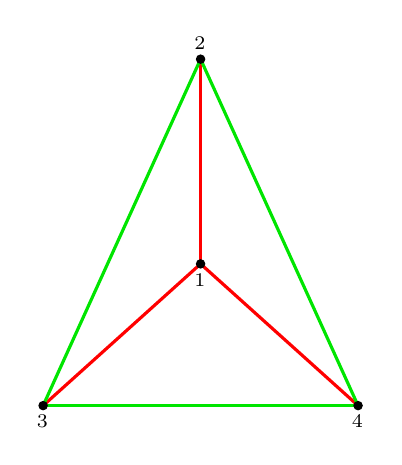
\begin{tikzpicture}
        % coordinates
        \coordinate (x1) at (0,-0.5);
        \coordinate (x2) at (0,2.1);
        \coordinate (x3) at (-2,-2.3);
        \coordinate (x4) at (2, -2.3);
        % boundaries
        \draw[line width=0.4mm, red] (x1) -- (x2);
        \draw[line width=0.4mm, red] (x1) -- (x3);
        \draw[line width=0.4mm, red] (x1) -- (x4);
        \draw[line width=0.4mm, black!10!green] (x2) -- (x3);
        \draw[line width=0.4mm, black!10!green] (x3) -- (x4);
        \draw[line width=0.4mm, black!10!green] (x2) -- (x4);
        
        % vertices
        \filldraw [black] (x1) circle (1.5pt);
        \filldraw [black] (x2) circle (1.5pt);
        \filldraw [black] (x3) circle (1.5pt);
        \filldraw [black] (x4) circle (1.5pt);
        
        %%%%%%%%%%%%%%%%%%%%%%%%%%%%%%%%%%%%%%%%%%%%%
        % % coordinates
        % \coordinate (x12) at (x1);
        % \coordinate (x22) at ($(x2)!0.3!(x1)$);
        % \coordinate (x32) at ($(x3)!0.3!(x1)$);
        % \coordinate (x42) at ($(x4)!0.3!(x1)$);
        % % boundaries
        % % \draw[line width=0.4mm, red] (x12) -- (x22);
        % % \draw[line width=0.4mm, red] (x12) -- (x32);
        % % \draw[line width=0.4mm, red] (x12) -- (x42);
        % \draw[line width=0.4mm, black!10!blue] (x22) -- (x32);
        % \draw[line width=0.4mm, black!10!blue] (x32) -- (x42);
        % \draw[line width=0.4mm, black!10!blue] (x22) -- (x42);
        
        % % vertices
        % \filldraw [black] (x12) circle (1.5pt);
        % \filldraw [black] (x22) circle (1.5pt);
        % \filldraw [black] (x32) circle (1.5pt);
        % \filldraw [black] (x42) circle (1.5pt);
        
        % Text
        \node[draw=none, color=black, below] at (x1) {$\x_{1}$};
        \node[draw=none, color=black, above] at (x2) {$\x_{2}$};
        \node[draw=none, color=black, below] at (x3) {$\x_{3}$};
        \node[draw=none, color=black, below] at (x4) {$\x_{4}$};
        
        % % Text
        % \node[draw=none, color=black, right] at (x22) {$\widetilde{\x}_{2}$};
        % \node[draw=none, color=black, below] at (x32) {$\widetilde{\x}_{3}$};
        % \node[draw=none, color=black, below] at (x42) {$\widetilde{\x}_{4}$};
        
    \end{tikzpicture}
    \label{fig:delta2_1}
    }\hspace{5em}
    \subfloat[$\Delta E^{\triangle}_0$] {    
    \begin{tikzpicture}
        % coordinates
        \coordinate (x1) at (0,-0.5);
        \coordinate (x2) at (0,2.1);
        \coordinate (x3) at (-2,-2.3);
        \coordinate (x4) at (2, -2.3);
        
        % \draw[line width=0.4mm, black!10!green] (x2) -- (x3);
        % \draw[line width=0.4mm, black!10!green] (x3) -- (x4);
        % \draw[line width=0.4mm, black!10!green] (x2) -- (x4);
        
        % vertices
        \filldraw [black] (x1) circle (1.5pt);
        \filldraw [black] (x2) circle (1.5pt);
        \filldraw [black] (x3) circle (1.5pt);
        \filldraw [black] (x4) circle (1.5pt);
        
        %%%%%%%%%%%%%%%%%%%%%%%%%%%%%%%%%%%%%%%%%%%%%
        % coordinates
        \coordinate (x12) at (x1);
        \coordinate (x22) at ($(x2)!0.3!(x1)$);
        \coordinate (x32) at ($(x3)!0.3!(x1)$);
        \coordinate (x42) at ($(x4)!0.3!(x1)$);
        
        % boundaries
        \draw[line width=0.4mm, red] (x22) -- (x2);
        \draw[line width=0.4mm, red, dashed] (x1) -- (x22);
        \draw[line width=0.4mm, red] (x32) -- (x3);
        \draw[line width=0.4mm, red, dashed] (x1) -- (x32);
        \draw[line width=0.4mm, red] (x42) -- (x4);
        \draw[line width=0.4mm, red, dashed] (x1) -- (x42);
        % boundaries
        % \draw[line width=0.4mm, red] (x12) -- (x22);
        % \draw[line width=0.4mm, red] (x12) -- (x32);
        % \draw[line width=0.4mm, red] (x12) -- (x42);
        \draw[line width=0.4mm, black!10!green, dashed] (x22) -- (x32);
        \draw[line width=0.4mm, black!10!green, dashed] (x32) -- (x42);
        \draw[line width=0.4mm, black!10!green, dashed] (x22) -- (x42);
        
        % vertices
        \filldraw [black] (x12) circle (1.5pt);
        \filldraw [black] (x22) circle (1.5pt);
        \filldraw [black] (x32) circle (1.5pt);
        \filldraw [black] (x42) circle (1.5pt);
        
        % Text
        \node[draw=none, color=black, below] at (x1) {$\x_{1}$};
        \node[draw=none, color=black, above] at (x2) {$\x_{2}$};
        \node[draw=none, color=black, below] at (x3) {$\x_{3}$};
        \node[draw=none, color=black, below] at (x4) {$\x_{4}$};
        
        % Text
        \node[draw=none, color=black, right] at (x22) {$\widetilde{\x}_{2}$};
        \node[draw=none, color=black, below] at (x32) {$\widetilde{\x}_{3}$};
        \node[draw=none, color=black, below] at (x42) {$\widetilde{\x}_{4}$};
        
    \end{tikzpicture}
    \label{fig:delta2_2}
    }
    \caption{Sketch of energies for computing $\Delta^2 E^{\triangle}$, see Figure \ref{fig:SE_nucleation2}}
    \label{fig:delta2}
\end{figure}

\section{Numerical Experiments}

\emph{Comment: Just including explanation of the
experiment for now. More experiments should
come next after discussing which ones.}

Here we are including numerical experiment
with initially $2000$ grains, constant
distribution of stored energy equal $SE=6$
(due to Figure \ref{fig:SE_experiments} and numerical experiments related),
numerical domain $\Omega=[0,2]^2$
with periodic boundary conditions.

Notice, since the bound for maximum difference of
stored energy is an absolute value (it is $6$), 
we needed to increase the computational domain
so we were able to obtain $\Delta^2 E^{\triangle}<0$,
otherwise this is very unlikely.
If this constraint is not satisfied,
we have have triple junctions with dihedral
angles greater that $180^{\circ}$ and
those triple junctions could cross grain
boundaries and create a corrupt grain
network. This may be handled with newer
types of topological transition.

A numerical simulation can be observed
in Figure \ref{fig:nucleation_stages}.

\begin{figure}
\begin{tabular}{cc}
\vspace{-4em}
\subfloat{\includegraphics[scale=0.3]{figures/nucleation_ic.png}} & \subfloat{\includegraphics[scale=0.3]{figures/nucleation_gg.png}} \\
\vspace{-4em}
\subfloat{\includegraphics[scale=0.3]{figures/nucleation_first.png}} & \subfloat{\includegraphics[scale=0.3]{figures/nucleation_second.png}} \\
\vspace{-4em}
\subfloat{\includegraphics[scale=0.3]{figures/nucleation_third.png}} & \subfloat{\includegraphics[scale=0.3]{figures/nucleation_final.png}}
\end{tabular}
\label{fig:nucleation_stages}
%\caption{Grain Growth and Recrystallization}
\end{figure}
